\documentclass{article}

\usepackage{fancyhdr}
\usepackage{ragged2e}
\usepackage{graphicx}
\usepackage{caption}
\usepackage{geometry}
\usepackage{amsmath}
\usepackage{rotating}

\usepackage{listings}
\usepackage{color}

\definecolor{dkgreen}{rgb}{0,0.6,0}
\definecolor{gray}{rgb}{0.5,0.5,0.5}
\definecolor{mauve}{rgb}{0.58,0,0.82}

\lstset{frame=tb,
  language=Java,
  aboveskip=3mm,
  belowskip=3mm,
  showstringspaces=false,
  columns=flexible,
  basicstyle={\small\ttfamily},
  numbers=none,
  numberstyle=\tiny\color{gray},
  keywordstyle=\color{blue},
  commentstyle=\color{dkgreen},
  stringstyle=\color{mauve},
  breaklines=true,
  breakatwhitespace=true,
  tabsize=4
}

\setcounter{secnumdepth}{1}

\usepackage{chngcntr}
\counterwithin{figure}{section}

\renewcommand*{\thepage}{C\arabic{page}}

\pagestyle{fancy}
\lhead{ACME Robotics}
\chead{\#8367}
\rhead{\ifcontents Contents \else Week \thesection \fi}

\newif\ifcontents
\contentstrue

\makeatletter
\renewcommand{\@seccntformat}[1]{}
\makeatother

\begin{document}\contentsfalse
\subsection{Add finishing touches to the Business Notebook}
%! Finish the Appendices and do a final read through of the Business Notebook.
The final part of the Business Notebook was writing the Appendices. The Appendices are very important because they include all of the extra information that doesn't fit other sections in the notebook. For example the fundraising letters are put in to the appendix because they are very long and don't fit perfectly in the section where fundraising and sending the letters is mentioned. Therefore, they are referenced in those places but the real letters are at the back of the notebook. This is the same story for the budget details. There is a general budget in the budget section but the individual purchases are in the appendix. \\
The final thing to do with the BN is to read through it once more, fix typos, add a few more photos and print the notebook. Emma took team and mentor photos for the bios and then a team photo for the "team" section. After that was done, she downloaded the BN PDF and printed the notebook. There are still a few things to add in order for the notebook to be completely done, such as write the summary page and space out the sections with dividers, but the goal to print the notebook at least a day before the tournament was met!

\subsection{ACME Board}
%! Finish the pit board that the team is going to take to the Burlingame tournament.
This week, Ben was tasked with making the ACME board. To do this he typed up multiple short paragraphs about subsystems, outreach, and software. Then he printed them out along with photos that show a visual. In Figure \ref{fig:pitboard} you can see the sketch that Ben made of the layout of the board. 

\begin{figure}
    \centering
    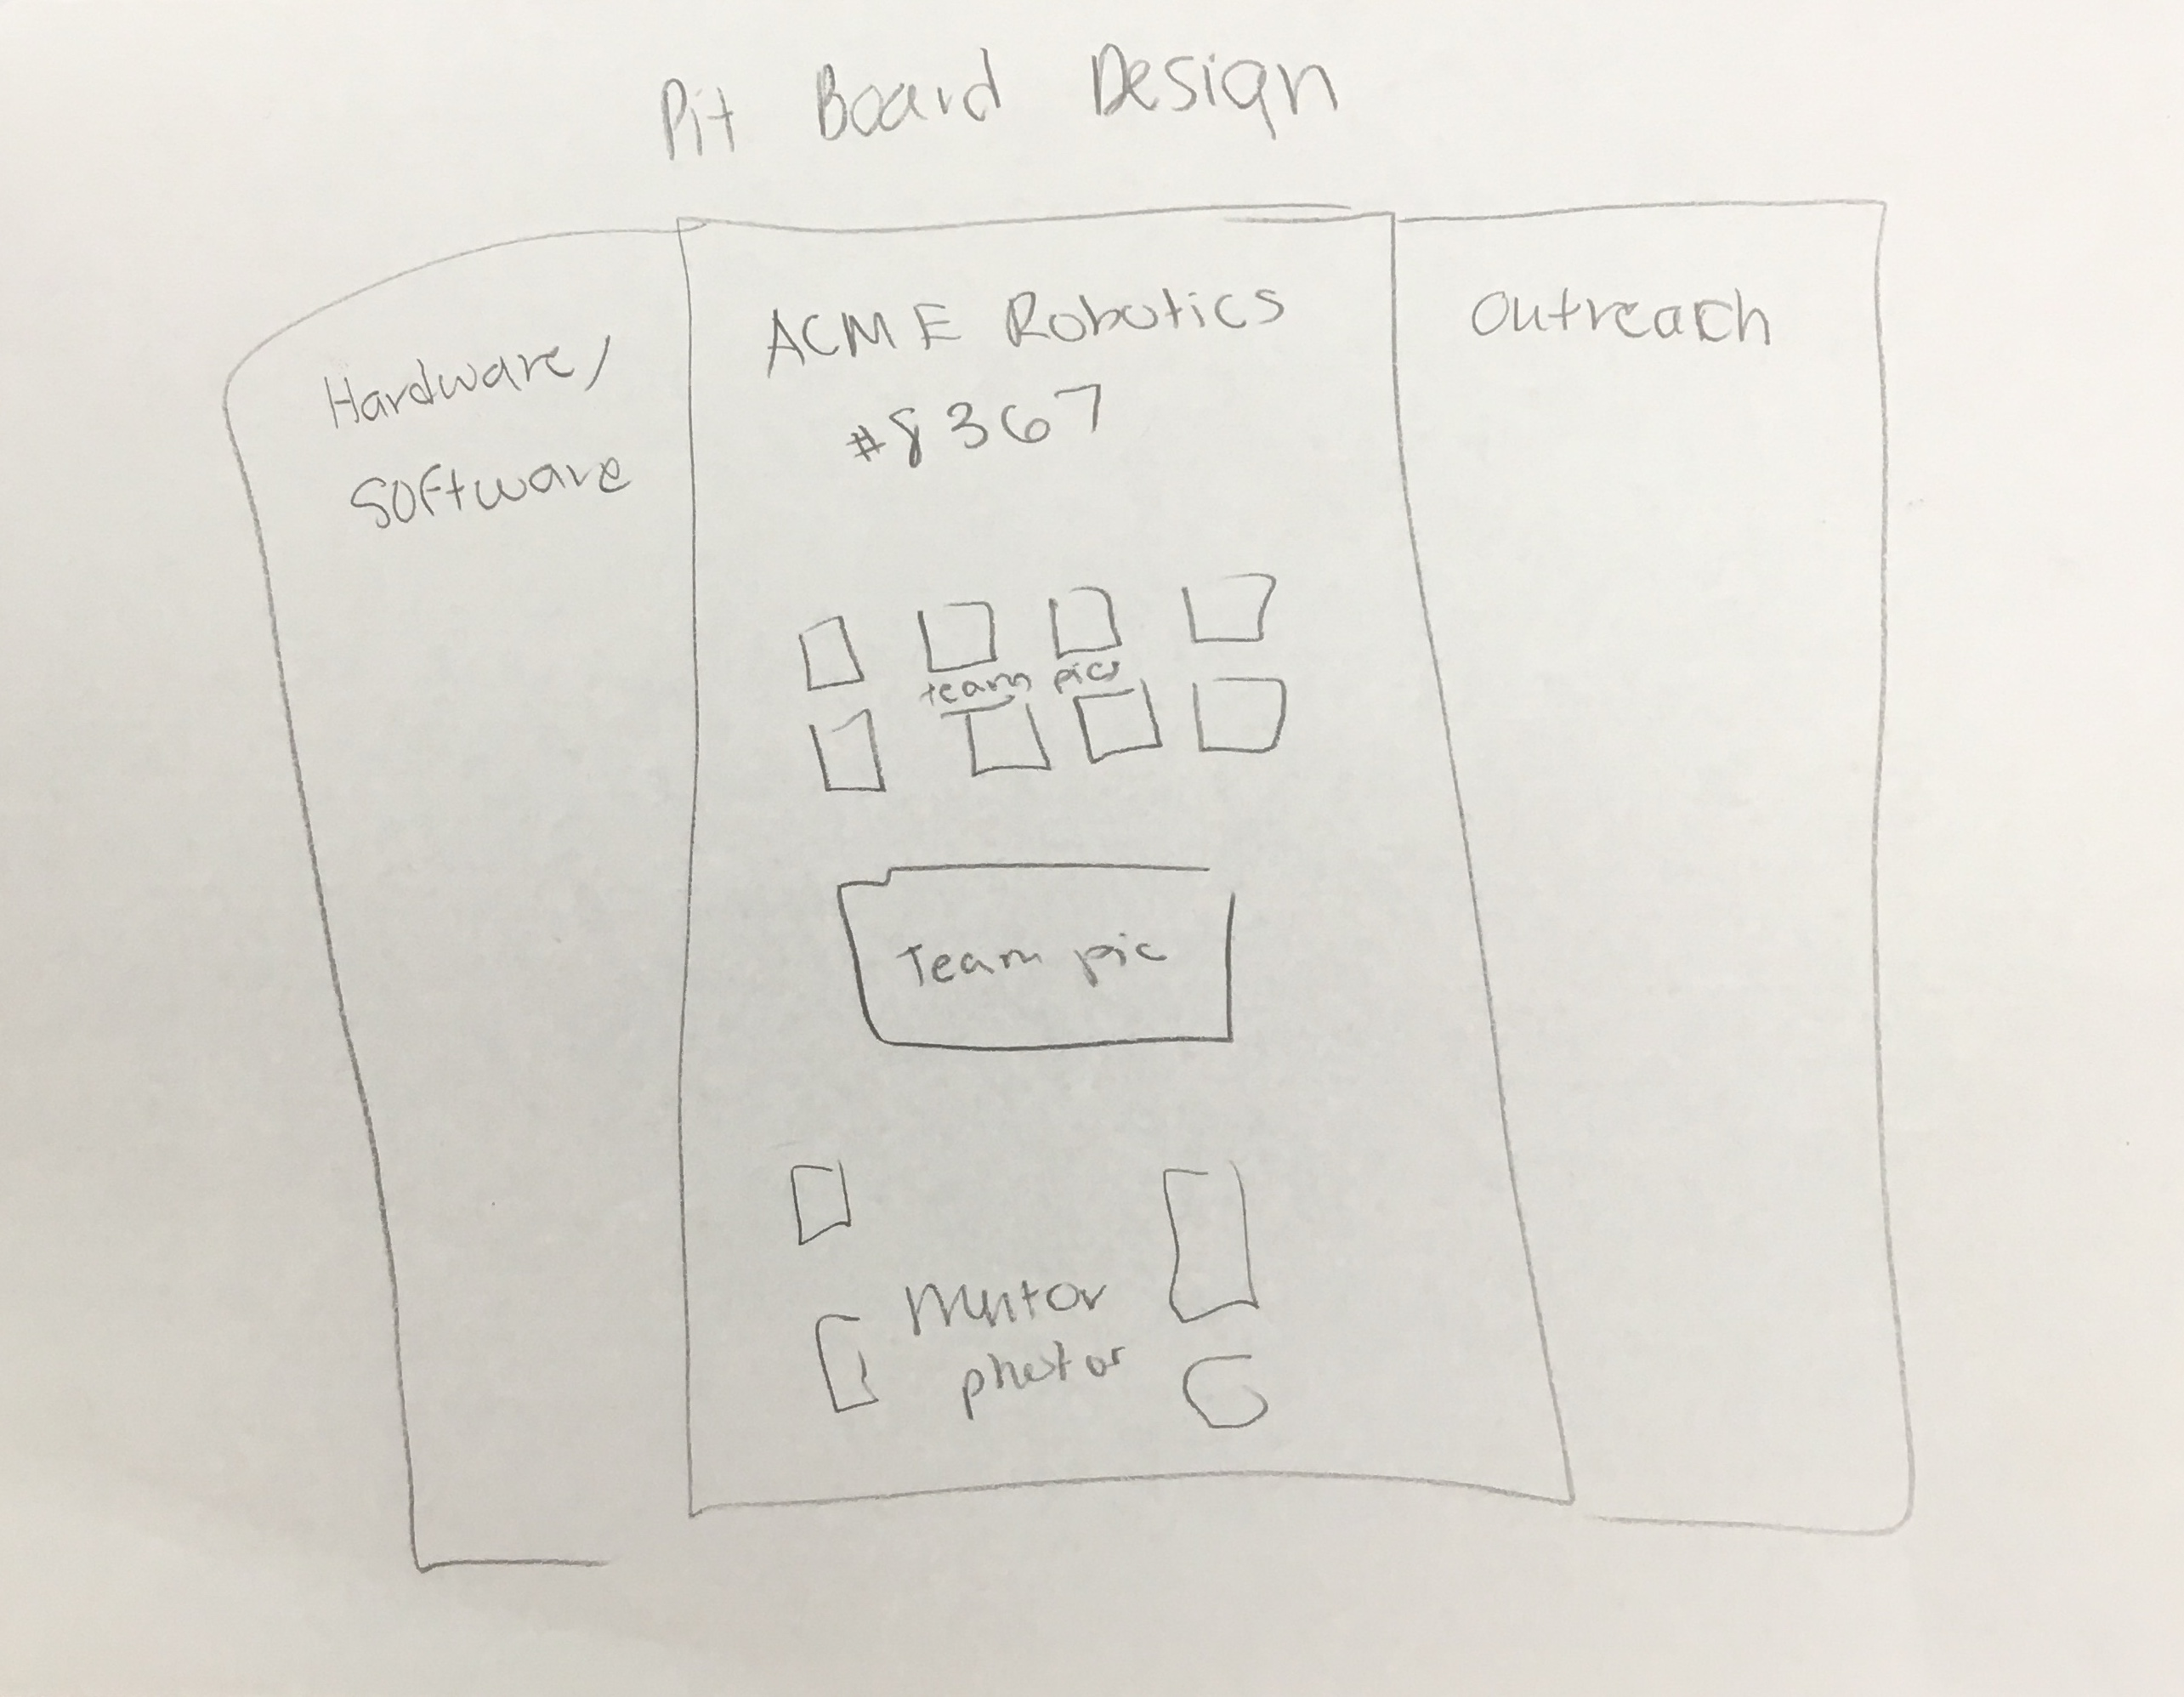
\includegraphics[width=.6 \textwidth]{10_11-05/images/pit_board.jpg}
    \caption{Pit Board Sketch}
    \label{fig:pitboard}
\end{figure}

\end{document}